%\documentclass[12pt,oneside]{book}
\documentclass[12pt]{book}
%\usepackage[paperwidth=6in,paperheight=9in]{geometry}
\usepackage[a4paper]{geometry}
%\usepackage[]{geometry}
\usepackage{style/style,style/tlfour,style/tlfive,style/bibAndIndex}
\bibliography{tex/bib/refMan.bib}
%\makeindex[intoc]
% \renewcommand*{\marginfont}{\color{NavyBlue}\bfseries\sffamily}
%
%For Table of Contents
\setcounter{tocdepth}{1}
\usepackage{tocloft}
\setlength{\cftsecnumwidth}{4em}
\makeatother
\begin{document}
    \frontmatter
	\begin{titlepage}
	\centering
%	\includegraphics[width=0.15\textwidth]{example-image-1x1}\par\vspace{1cm}
	{\scshape\LARGE TrainABA Supervision Curriculum Series\par}
	\vspace{1cm}
	{\scshape\Large Volume 1: BCBA Reference Manual\par}
	\vspace{1.5cm}
	{\huge\bfseries Fifth Edition\par}
	\vspace{2cm}
	{\Large\itshape Ben Theisen\par}
	\vfill
	Free and Open Source Community Edition \par   
	Cumulative Records Documentation Society

	\vfill

% Bottom of the page
	{\large \today\par}
\end{titlepage}

		\null \vfill
	\noindent%
		Copyright $\copyright$ 2019. Second Edition. \\
		Updated: \today. \\
	\noindent%
		This book may be downloaded as a free PDF at (website).
		This textbook is also available under a Creative Commons license.
		Source files hosted on {Github}. \\

	\noindent Los Angeles, California, USA.
	\clearpage

	\clearpage
	\tableofcontents
	\clearpage
	\listoffigures
	\clearpage
	\listoftables
	\clearpage
	\chapter{About the Maintainer}
%\noindent {\Huge About the Maintainer\par}

This book is maintained by Ben Theisen. He earned a PhD in Business Psychology and MBA. He has been a Board Certified Behavior Analyst (\#1-10-7323) since 2010. Dr. Theisen is an adjunct professor in the Industrial-Organizational/Business Psychology Department at The Chicago School of Professional Psychology, Los Angeles Campus. He researches occupational characteristics of behavior analysis supervisors. He operates a private practice for behavioral and personnel consulting. His hobby is computer programming.
\clearpage

	\noindent {\Huge Preface\par}
This book is a labor of love. It serves as an excuse to incorporate GNU/Linux command line tools into the soul-crushing Microsoft workflow of many behavioral service providers. 

Anyone is welcome to participate in the development of this book and other projects like it. All of the source code, including the latest PDF version, is publicly available. 

The code is maintained through Cumulative Records Documentation Society (CRDS), a 501c3 nonprofit. GitHub, a software development organization, has generously provided CRDS with lifelong sponsorship for projects like this one.

The technology choices for this book were a form of artistic expression. These tools promote community in the century-long development of behavior analytic services as a profession. The act of using these tools was meant to be rebellious, if not subversive, against the way large books are usually developed. The technology  for this book reflected the do-it-yourself spirit of Skinner's hands-on work with operant chambers. It was pure hip-hop with two turntables and a sampler. It was grunge rock singing love songs in an old garage. It was a \$200 single-subject design study at a university where other departments held out for seven figure grants.

The computers used to build this book were a nod to the traditional applied behavior analysis studies, which could be conducted for cheap with a clipboard and some doctoral students. The best example was an old Lenovo ThinkPad X200, purchased second-hand from Craigslist with cash. This was a statement against consumerism. It said no to ``upgrading" to next-generation CPUs that ran the telemetry nightmare known as Windows 10.

For this statement, the X200 was perfect. It was golden-era hip hop in all its sound sampling glory. The laptop had a battery life of 23 minutes and came pre-installed with Hello Kitty stickers on certain keys. The stickers said things like, ``return," ``shift," and ``a." And yes, all stickers were placed correctly. The X200 ran a free and open source operating systems powered by GNU/Linux and approved by the Free Software Foundation.

This book was proudly typeset using \LaTeX, a free and open source software (FOSS). FOSS was chosen as a nod to B.F. Skinner's writings on culture, in which he voiced the difficulties of communicating non-physical technologies to new audiences. Rather than create a book to be released on a bookshelf, this book was designed from publicly available code. The version control notes were public, so anyone could see the process of creating the book. The goal of these tools was to add a layer of physical technology to a book whose subject was a non-physical technology. Hence, it built on Skinner's vision of better communicating the technology of behavior analysis to general audiences.

\LaTeX allowed modularization of the book's files. It keeps all the writing separate from the files that generate the formatting. This was a nod to the stories of Skinner's lab. As the legends tell, one could hear the operant chambers clacking from various experiments, happening simultaneously though measured and analyzed as separate phenomena. In this book's modular design, each file held its own content. Any content file could easily be removed, modified, or replaced without any impact on other pages.


The books were assembled and written using Vim, a free and open source command line text editor. It was compiled using custom shell scripts in a Bash terminal. Git and GitHub were used for version control. The decision to use a command line editor was a nod to an operant chamber. One need only peck at the keys to write, assemble, and distribute this book. No mouse, trackpad, eyes, or graphic user interface is involved. An experienced operator could complete the process blindfolded. The author suffers from tendonitis and frequent eyestrain from extensive computer use, so the command line technology is a welcome option.


While the specifics of the technology choices for this book may seem gratuitous, the purpose was to inspire behavior analysis professionals to indulge their curiosity in computer programming. The intended message is, roughly, that even an English major can learn to write code if the project is interesting. Perhaps others from non-programming backgrounds will consider this project as an invitation to download and tinker with code.

Please submit errors, additions, improvements, and suggested omissiongs using the GitHub Issue Tracker. Nothing posted in the modern day mead-halls of Facebook Groups will be read by those who maintain this book.

All readers may use, copy, modify, and distribute this book and its files. Hard copies are available. Custom builds are available for companies, universities, and others. Please contact CRDS for more information about how to use intellectual property for this book or make content contributions. The contact is postmaster(at)cumulativerecords.org.

The Behavior Analyst Certification Board provided a copyright license for use of the BCBA/BCaBA Task List, 4th and 5th editions. No reprinting of those materials are allowed without the express written consent of the BCBA/BCaBA. Statements of free and open source licensing of this book do not apply to the BCBA/BCaBA Task List, which is the sole property of the Behavior Analyst Certification Board. For more information, visit www.bacb.com.

Some of the content in this book builds upon work from contributors to its first edition. This book represents significant revision, rewriting, and reorganization, to the point that it is a completely different book representing original content. The first edition continues to be available through the GitHub repositories. It has been made publicly available under a Creative Commons 4.0 - Attribution - Sharealike - Noncommercial license since 2017.
\clearpage

%	\noindent {\Huge About the Second Edition\par}
\begin{displayquote}
\textit{This book was made by GNU/Linux computers, under supervision of a BCBA.}
\end{displayquote}
The second edition has advantages over the first. Its user license guarantees the freedoms specified under the Creative Commons 4.0 - Attribution - Sharealike - Non-commercial (CC 4.0-BY-SA-NC). The license provides readers with the freedom to use, copy, modify, and distribute the book non-commercially. This is a good thing for behavior analysts because we like to customize everything. Modified and copied versions retain the same freedoms as the original work. There is no need to ask the publisher for permission to reprint the book's contents. 

However, no amount of licensing is useful if users have difficulty accessing the full manuscript text in an editable format. This version uses a typesetting system that users can easily customize. It is maintained by Cumulative Records Documentation Society (CRDS), a 501(c)(3) nonprofit. The nonprofit has secured a lifelong sponsorship from GitHub to host the full manuscript and source code. This means you can re-brand with your company name, change the contents or sections, etc. It also means the book can be improved by creating an Issue in GitHub, which a maintainer from the nonprofit can address. Such changes will improve the main version of the book, distributed to all. All previous versions will remain available. The technology has incredible applications for behavior analysts. CRDS is a BACB-authorized continuing education provider and will offer workshops to help users take advantage of these capabilities.

These advancements make the second edition far superior to the traditional ``all rights reserved'' copyright used in the first edition printings. This edition also offers superior typesetting technology. Content is better due to richer connections to the literature, more performance measures for assessment, and more generality in examples.

The book is distributed freely with paper copies sold at a reasonable price. The profits go to a public charity (CRDS) to advance the contents of the book.

\section{History of the TrainABA Supervision Curriculum Series}
This book originated from a project from TrainABA, a startup organization from 2013-2016. Its goal was to function as a publisher and resource for behavior analysis supervision. It was unsuccessful. When TrainABA closed, the publisher released its works under a Creative Commons 4.0 - Attribution - Sharealike - Non-commercial license. Some of its works survived as a project, such as the free Moodle Course, manuscripts, and SAFMEDs app. These works were donated to CRDS to be developed as a community edition for public use. 

\section{Publisher}
The publisher is CRDS, a 501(c)(3) nonprofit based in Los Angeles, California, USA. CRDS produces archive-quality continuing education materials for public use. CRDS employs technical producers and project maintainers to develop and distribute works. CRDS survives on the generosity of its members. If your company uses these materials, we ask that you donate a reasonable amount to support the cause. The donation is to make sure these high-quality materials will continue to be available to your company in the future. To make a donation, or to become a member, please visit \url{http://cumulativerecords.org}.

\section{Collaboration Tools}
CRDS built this book using collaboration tools from software developers. Anyone can contribute or suggest changes for free. There will be a permanent public record of any such collaboration. We encourage readers to report errors using the Issue Tracker on our GitHub repository. The location is: \url{https://github.com/cumulativerecords/trainaba-v1-ed2/issues}

\subsection{Creating New Materials from This Book}
Readers can and should extend the book's contents (e.g., build a slideshow to be used where one works or teaches). All readers are invited to suggest changes to this book using the GitHub repository. For readers who have modified the contents to be used where they work or teach, we ask that you submit your materials to CRDS so that we can make them available to other readers. We believe this will afford us the opportunity to have one or two well-developed versions of a work, which are compatible with the original book. We believe one organized version is better than multiple partially-developed, incompatible but similar works. 

%Readers who create materials retain credit for their contributions. In many cases, CRDS will supply content creators with a technical producer who will help them organize the materials for larger audiences at no charge. Organizations who use CRDS materials regularly for personnel development provide donations.

%\subsection{Online Documentation}
%The materials in this book will likely be distributed as online documentation from \url{https://ReadTheDocs.org}. More information about this project will be made available at a later release. 

\section{Versions}
The typesetting system used to compile this work is very flexible. It can compile a similar version for nearly any page size with a very simple change in code. It is designed to provide maximum flexibility to readers, who are often supervisors and educators with a need to use only certain sections of this work. By downloading the source code, readers are able to pick and choose which sections of the book to compile. They can rebrand the book to indicate that they modified the original version. Readers are invited to tinker with the source code to download modified versions of the work. It is surprisingly easy to make a mobile-friendly version of this book, for example. One can also make a new version for each month in a supervision setting. CRDS is available to provide customizations for organizations and universities. To request a custom version, contact CRDS at \url{http://cumulativerecords.org/contact}.





%	\chapter{Administration}
This is a whole chapter about administration for supervisors. None of it is dependent on implementing procedures of certification or licensing entitities. For example, \underline{\texttt{\colorbox{Dandelion}{Fourier series}}}
%\marginnote{Fourier Series}
\index{Fourier series}
gets indexed for no apparent reason.

Say, do you remember that image of space from last chapter? Here is the image, presented as a figure. Look how pretty a figure can be!
\begin{figure}[h]
    \centering
    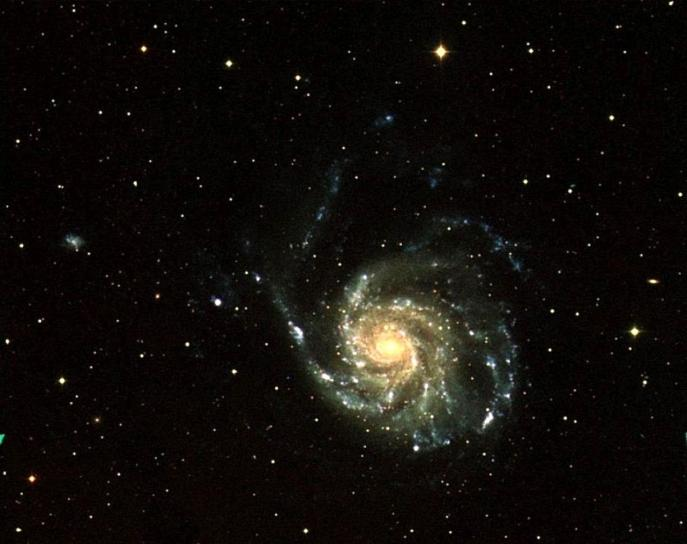
\includegraphics[width=0.25\textwidth]{space}
    \caption{A nice space.}
    \label{fig:space1}
\end{figure}
 
As you can see in the figure \ref{fig:space1}, the 
function grows near 0. Also, in the page \pageref{fig:space1} 
is the same example.
 
All of this continues to another page, which includes a bulleted list.
\begin{itemize}
\item fun
\item sun 
\item rock
\item roll
\item okay
\end{itemize}

The most important consideration is the use of power when microwaving burritos. Whether at a concert or anywhere that sells gasoline, burritos and microwaves are your friends. These are the friends you want to keep. Parents encourage their kids to have these lasting relationships. 

It's never too early to start thinking about tabular presentation of data. Yes, we're talking tables.

\section{Behavioral Data Table}
\begin{table}[H]
\begin{tabular}{|l|cccccc|}
\hline
\multicolumn{1}{|c|}{Behavior} & AR18 & Q1 & Q2 & Goal & Change & Met?\\\hline
Physical Aggression            & 0    & 0  & 0  & 0    & +      & No\\
Self-Harm                      & 0    & 0  & 0  & 0    & +      & No\\
AWOL                           & 0    & 0  & 0  & 0    & -      & Yes\\
Fabricating Stories            & 0    & 0  & 0  & 0    & -      & Partial\\ \hline
\end{tabular}
%THE LIST OF TABLES ONLY LISTS CAPTIONS.
%PLACE A CAPTION AFTER THE \end{tabular}.
\captionof{table}{A simple behavioral data table}\label{tbl:simplebehavioral}
\end{table}


A \textcolor{orange}{TikZ}
%\marginnote{TiKZ} 
\index{TikZ}
 figure will be rendered below this line. It has to get to the next page first. Be sure to hold your excitement for the moment. It really will be ready to show momentarily. Any old moment. Could be this one. Maybe now? 
 \begin{figure}[ht]
 \subimport{../}{diagram/diagram.tex}
 \label{fig:tikzexample}
\caption{A nice simple diagram}
\end{figure}





    \mainmatter
%	Write chapters below.
	\import{tex/chapters/fourth-ed/intro/}{intro.tex}
	\import{tex/chapters/fourth-ed/}{fourseca.tex}
	\import{tex/chapters/fourth-ed/}{foursecb.tex}
	\import{tex/chapters/fourth-ed/}{foursecc.tex}
	\import{tex/chapters/fourth-ed/}{foursecd.tex}
	\import{tex/chapters/fourth-ed/}{foursece.tex}
	\import{tex/chapters/fourth-ed/}{foursecf.tex}
	\import{tex/chapters/fourth-ed/}{foursecg.tex}
	\import{tex/chapters/fourth-ed/}{foursech.tex}
	\import{tex/chapters/fourth-ed/}{fourseci.tex}
	\import{tex/chapters/fourth-ed/}{foursecj.tex}
	\import{tex/chapters/fourth-ed/}{fourseck.tex}
	\import{tex/chapters/fourth-ed/}{foursecFK.tex}
	\import{tex/chapters/fourth-ed/after-internship/}{after-internship.tex}
		
	\documentclass{book}
\usepackage{glossaries}
\makeglossaries
%%%%%%%%%%%%%%%%%%%%%%%%%%%%%%%%%%%%%%%%%%%%%%%%%%%%%%%%%%%%%%%%%
%								%
%BEGIN GLOSSARY ENTRIES						%
%								%
%%%%%%%%%%%%%%%%%%%%%%%%%%%%%%%%%%%%%%%%%%%%%%%%%%%%%%%%%%%%%%%%%

\newacronym{cat}{CAT}{A sleepy animal}

%TERMS: 
%LABEL = What LaTeX calls this entry.
%NAME = What readers see as a name for entry.
%DESCRIPTION = What readers see as explanation for the term.
%\newglossaryentry{label}
%{
%name={name},
%description={description},
%other options
%}
%FOR LONG GLOSSARY ENTRY, USE \longnewglossaryentry. It allows paragraph breaks.

\newglossaryentry{behavior}
{
	name = {Behavior},
	description = {Refers to an observable act or response from a living organism}
}

\newglossaryentry{applied}
{
	name = {Applied},
	description = {Refers to selection of socially significant behaviors when designing interventions}
}

%%%%%%%%%%%%%%%%%%%%%%%%%%%%%%%%%%%%%%%%%%%%%%%%%%%%%%%%%%%%%%%%%
%								%
%END GLOSSARY ENTRIES						%
%								%
%%%%%%%%%%%%%%%%%%%%%%%%%%%%%%%%%%%%%%%%%%%%%%%%%%%%%%%%%%%%%%%%%


\begin{document}
%\chapter{Glossary}
\glsaddall
\printglossary[nonumberlist]
%\clearpage


%\gls{cat}


\end{document}

	\nocite{*}
	\printbibliography[title=References,heading=bibintoc]
% Print the printbibliography.
% Now print indexes.
\raggedright
\printindex         % the general index
\printindex[names]  % the name index
\printindex[titles] % the title index   
\end{document}
